\documentclass{article}
\usepackage{graphicx}
\usepackage{epstopdf}
\usepackage{natbib}
\usepackage{multirow}
\usepackage{amsmath}
\usepackage[dvipsnames]{xcolor}
\usepackage{hyperref}
\usepackage{float} % Needed to force figure dump in specific location. Use [H] option.
\usepackage[left=1in, right=1in, top=1in, bottom=1in]{geometry}
\usepackage{titlesec}
\usepackage[percent]{overpic}
\usepackage{contour}
\usepackage{array}
\usepackage{tabularx}

\newcommand{\genDisc}[1]{\medskip \hrule \vspace{0.25cm}
               {\itshape {\color{violet}{#1}\color{black}} }}
               
\newcommand{\pointRaised}[2]{\medskip \hrule \vspace{0.25cm}
               {\itshape {\bfseries \color{violet}{#1}}: \color{violet}{#2}\color{black}}}
               
\newcommand{\pointRaisedNoRef}[1]{\medskip \hrule \vspace{0.25cm}
               {\itshape {\color{violet}{#1}\color{black}} }}

\newcommand{\reply}{\vspace{0.25cm} \textbf{Reply}:\ }

\newcommand{\zeply}[1]{\vspace{0.25cm} \color{red}\textbf{Reply}:\ {#1}\color{black}}

\newcommand{\todo}[1]{\textcolor{red}{#1}}

\newcommand{\degree}{$^{\circ}$}

\renewcommand{\thefigure}{R\arabic{figure}}
\renewcommand{\thetable}{R\arabic{table}}

\begin{document}

\title{Author Response to Reviewer \#2 of egusphere-2023-3094, `Algorithmically Detected Rain-on-Snow Flood Events in Different Climate Datasets: A Case Study of the Susquehanna River Basin'}
\author{Colin M. Zarzycki, Benjamin D. Ascher, Alan M. Rhoades, and Rachel R. McCrary}
\date{}

\maketitle
\pagenumbering{gobble}

Specific responses regarding Reviewer \#2's comments are contained in the text that follows. We have highlighted in {\color{Orange}areas in orange} (chosen for color blindness) where we have further refined the manuscript in response to these comments.

\subsection*{Response to Reviewer \#2}

\genDisc{The authors present an inter-model comparison of basin-scale rain-on-snow (RoS) flood events identified using different detection algorithms for a 21-year historical period over the Susquehanna River Basin, located in the eastern US. Compared to observations, the algorithm flags known historical events, but there are model-specific discrepancies in terms of event magnitude and the driving factors of precipitation, runoff, snowpack, and snowmelt contribution. The authors report that the use of dataset-specific thresholds improves agreement between models but does not account for all discrepancies, which are attributed to differences in model structure, meteorological forcing, and coupling frequency.

The paper is well-written and clearly structured. The references cited are complete and up to date. The results are relevant to local and regional flood risk assessments using gridded climate and hydrometeorological data sets that are available at continental to global scales.

I have two general comments and a few detailed edits.
}

\reply{Thank you for your time and consideration in this review, please see our responses below, which we hope address all of this point-by-point and reflect an improved manuscript.}

\genDisc{It is mentioned that the ROF differences among hydrologic models can be extremely variable, with regional differences between products reaching an order of magnitude. Is this due to soil parameterization in models that influences infiltration capacity? Is there a difference in soil parameterization that sets L15 apart from the other models? Given the high uncertainty in soil parameterization, I wonder if there is benefit in including ROF as a threshold.

There is a misunderstanding evident on Line 125. The statement ``20\% reduction in the snowpack (implied dSWE $<=$  -20 mm/day)'' is incorrect. The 20\% snowmelt contribution threshold applied by Freudiger et al. (2014), which was subsequently adopted by Musselman et al. (2018) and Li et al. (2019), is described as: ``... for which the sum of rainfall and snowmelt contains a minimum of 20\% snowmelt.'' This is a key point to make clear. What is helpful about this threshold condition is that it doesn’t rely on characterization of soil infiltration capacity, which is difficult to validate in models and can vary over an order of magnitude regionally and between models.

What I like about your inclusion of the ROF variable is that it connects to the importance of antecedent soil moisture and saturated conditions to driving flood response. More discussion on this topic is probably warranted. Requiring ROF$>$0 is a condition that the soil must be saturated to result in flood, which is intuitive, and then not surprising that the flagged events in the simulations correspond to streamflow events in the USGS record.

Given that (at least) these three papers adopted the ``20\%'' threshold to identify times when snowmelt is substantially contributing to rainfall + snowmelt fluxes, I encourage the authors to include this 20\% value in their FIXED (and X\% in their RELATIVE) analyses. Given the uncertainty associated with estimating ROF, can you identify flood events in the record without requiring ROF? What is potentially missed / lost if one doesn’t include ROF? For example, excluding ROF as a condition is analogous to not knowing the buffering capacity of soil water deficit. Would that impact the ability of an automated algorithm to flag potentially impactful RoS events? This would seem to be an important tie to previous studies – because I do think antecedent soil saturation is important - and could result in key guidance to future research efforts.
}

\reply{
The mischaracterization of \citet{freudiger2014large} is a somewhat embarrassing oversight on our part. We have updated the text to reflect the criterion that at least 20\% of the sum of snowmelt and rainfall must come from snowfall (we note that the ratio of rainfall to snowmelt cannot exceed 4:1, which is mathematically identical).

We appreciate the suggestion. Because this is an interesting question, we have performed a sensitivity analysis where we also impose this threshold in our algorithm. We define a new threshold $t_{\textrm{fSWE}}$ equal to 0.2, which is computed as dSWE (sign flipped for snowmelt to be positive) divided by the sum of dSWE and PRECIP. As with the other three thresholds, $t_{\textrm{fSWE}}$ must be satisfied in our sensitivity run (RELATIVE\_F14). We find that for three of the four datasets, there is no change in the number of events. The one dataset that sees reduced event frequency is NLDAS, a product that shows high climatological PRECIP and low climatological SWE (and dSWE) over the SRB. Even though event frequency is the same we see a slight reduction in event length and average ROF in the other three datasets, implying that some days at event onset or event termination are removed when $t_{\textrm{fSWE}}$ is used.

We add these results to the text for readers.

{\color{Orange}
We also perform a sensitivity analysis intended to include the requirement in \citet{freudiger2014large} and \citet{musselman2018projected} that the sum of rainfall and snowmelt contains at least 20\% snowmelt.
This is added as an additional threshold $t_{\textrm{fSWE}}$ = 0.2 where fSWE (fraction of dSWE contribution) is computed as dSWE divided by the sum of dSWE and PRECIP smoothed time series (note, the sign of dSWE is inverted to be a positive contributor to liquid water on the surface).
We refer to this simulation as RELATIVE\_F14 since it preserves the same thresholds in RELATIVE with this one additional exclusionary check from \citet{freudiger2014large} in order to remove high rainfall (but low snow loss) events.
The number of events is the same for all datasets except NLDAS, which loses 7 events over the study period when enforcing $t_{\textrm{fSWE}}$ = 0.2.
This can be explained by the results in Fig. 2. NLDAS produces a `wetter' precipitation climatology (Fig. 2f) but less climatological SWE (Fig. 2j) and, correspondingly, less dSWE (Fig. 2n).
Therefore, enforcing a check that removes high PRECIP, low dSWE events would reduce events detected in NLDAS most strongly relative to other datasets.
While the other three products have the same number of events with or without the inclusion of $t_{\textrm{fSWE}}$ = 0.2, the mean duration is slightly shortened, and mean event ROF is somewhat reduced using RELATIVE\_F14, implying that a handful of high PRECIP, low dSWE (and high ROF) days at event onset or termination are lost.
However, this reduction is small and therefore provides confidence that just including threshold checks for dSWE, ROF, and PRECIP is satisfactory for detecting RoS events over the SRB without a more formal snow loss cutoff.
In the remainder of this paper, we omit the use of $t_{\textrm{fSWE}}$ for simplicity.
However, we want to emphasize that the simulation of land surface processes in different datasets can play a key role in precipitation/snowmelt partitioning, motivating further process-oriented evaluation of their joint occurrence in gridded climate data in the future.
A percentile-based threshold-only algorithm (such as RELATIVE) may particularly struggle in regions of climatologically low SWE and high PRECIP (which experiences primarily rain-induced flooding) or high SWE and low PRECIP (primarily melt-induced flooding).
}

\clearpage

The updated table reads:

\begin{table}[H]
\caption{Statistics of RoS events over the SRB using FIXED thresholds (top) and RELATIVE thresholds (bottom). $t_{\textrm{PRECIP}}$, $t_{\textrm{ROF}}$, and $t_{\textrm{dSWE}}$ represent the thresholds used for precipitation, surface runoff, and snow water equivalent loss, respectively (mm/day). Events represent the number of RoS events flagged over the 1980-2005 period. Duration is the average number of consecutive days an RoS event lasts. PRECIP$_{a}$, ROF$_{a}$, and dSWE$_{a}$ represent the amount of precipitation rate, amount of runoff rate, and average snow loss (mm/day) per event by calculating the mean daily value for each individual event and then averaging those.}
\scriptsize
\begin{tabular}{lccccccccc}
      &  $t_{\textrm{PRECIP}}$ & $t_{\textrm{ROF}}$ & $t_{\textrm{dSWE}}$ & $t_{\textrm{fSWE}}$ & Events & Duration & PRECIP$_{a}$ & ROF$_{a}$ & dSWE$_{a}$ \\
      &  \textit{mm day$^{-1}$} & \textit{mm day$^{-1}$} & \textit{mm day$^{-1}$} & \textit{\%} & \textit{\#} & \textit{days} & \textit{mm day$^{-1}$} & \textit{mm day$^{-1}$} & \textit{mm day$^{-1}$} \\ \hline
FIXED &         &         &         &        &     &              &              &                &                \\ \hline
L15 & 2.0 & 1.4 & -1.4 & - & 6 & 3.2 & 9.5 & 1.5 & -5.3 \\
NLDAS & 2.0 & 1.4 & -1.4 & - & 16 & 2.9 & 6.3 & 2.1 & -5.2 \\
JRA & 2.0 & 1.4 & -1.4 & - & 48 & 3.5 & 5.3 & 2.6 & -4.4 \\
E3SM & 2.0 & 1.4 & -1.4 & - & 58 & 4.1 & 6.5 & 2.4 & -5.2 \\ \hline
RELATIVE      &         &         &         &        &     &              &              &                &                \\ \hline
L15 & 2.0 & 0.6 & -1.5 & - & 20 & 5.2 & 6.2 & 1.1 & -5.3 \\
NLDAS & 2.0 & 1.4 & -0.8 & - & 20 & 2.8 & 7.2 & 2.1 & -4.2 \\
JRA & 2.0 & 1.6 & -1.9 & - & 40 & 3.1 & 5.1 & 2.5 & -4.1 \\
E3SM & 2.0 & 1.8 & -2.2 & - & 41 & 4.1 & 6.9 & 2.9 & -8.0 \\ \hline
RELATIVE\_F14      &         &         &         &        &     &              &              &                &                \\ \hline
L15 & 2.0 & 0.6 & -1.5 & 20 & 20 & 4.9 & 6.0 & 1.0 & -5.3 \\
NLDAS & 2.0 & 1.4 & -0.8 & 20 & 13 & 3.0 & 4.4 & 1.9 & -5.1 \\
JRA & 2.0 & 1.6 & -1.9 & 20 & 40 & 3.0 & 5.3 & 2.4 & -4.2 \\
E3SM & 2.0 & 1.8 & -2.2 & 20 & 41 & 4.0 & 6.8 & 2.8 & -7.8 \\   \hline
\end{tabular}
\label{table:means}
\end{table}

In general, we find that the algorithm is largely insensitive to this inclusion, although we add additional text suggesting further evaluation may be merited in different cases (for example, datasets and/or regions with a high frequency of ROF events arising from high PRECIP). In some ways, this -- to us -- implies using runoff and snowmelt is therefore implicitly enforcing events to contain high snowmelt fraction in a process sense. However, we choose not to speculate regarding that in the manuscript without further (future) investigation beyond the scope of this project.
}

\genDisc{It would be helpful to see more written about the transferability of the results to other regions / basins. Particularly, how transferrable would your results be to regions with more elevation complexity as it relates to model treatment of elevation-dependent hydrometeorology, snowpack, and soil antecedent conditions, which would seem relevant to the differences in model grid spacing? If not transferrable, could the authors provide guidance for future research efforts?
}

\reply{
This was also suggested by Reviewer \#1, so we have included a new section in the manuscript entitled {\color{Orange}`\textbf{Generalizability to other basins}.'} We have reproduced this new text in the Appendix of this response. In this section, we explore two basins in the US with notable RoS events (Willamette River Basin and Sacramento River Basin). Both basins contain more orographic complexity than the SRB. While only a cursory analysis, the algorithm did detect the largest RoS event over the study period in each basin. We find this result promising, although we also noted potential caveats and emphasized that this could be (an interesting!) target for future work, particularly for researchers interested in including ROF in RoS algorithms and/or exploring flood responses at the basin scale versus gridpoint values.
}

\genDisc{Line 181: ``(i.e., positive dSWE in both figures denotes snowpack)'', I think ``denotes snow accumulation'' is more accurate.}

\reply{Typo corrected.}

\genDisc{Line 225: This should be ``WY 1996''. In the US, the water year is designated by the calendar year in which it ends. The year ending September 30, 1996 is called the ``1996 WY'', which begins on Oct 1, 1995.}

\reply{Another embarrassing oversight. These have been corrected.}

\genDisc{Figures 2 \& 3: The histograms in panels b-d are very difficult for me to visually disentangle. Please consider making each variable-panel into 2x2 sub-panels showing the individual (solid / filled) colored histograms for each model.}

\reply{We agree that these plots were difficult to interpret. We liked this suggestion to create subpanels and it spurred an idea to convert these plots into 4x1 subpanels. We believe this does provide an improved interpretation of the previously overlapping plots. The updated version of Figure 3 is shown below.

\begin{figure}[H]
\begin{tabular}{cc}
\begin{overpic}[width=0.45\linewidth]{{figs/cropped/events_95}.pdf}
\put (11,72) {\contour{white}{\large a.}}
\end{overpic}
&
\begin{overpic}[width=0.45\linewidth]{{figs/cropped/Max_precip_95}.pdf}
\put (11,72) {\contour{white}{\large b.}}
\end{overpic}
\vspace{0.10cm} \\
\begin{overpic}[width=0.45\linewidth]{{figs/cropped/Max_runoff_95}.pdf}
\put (11,72) {\contour{white}{\large c.}}
\end{overpic}
&
\begin{overpic}[width=0.45\linewidth]{{figs/cropped/Max_dSWE_95}.pdf}
\put (11,72) {\contour{white}{\large d.}}
\end{overpic}
\end{tabular}
\caption{(Fig. 3 from manuscript) Same as Fig. 2 except for the RELATIVE detection thresholds.}
\label{fig:histograms}
\end{figure}

}

\genDisc{Thank you for the chance to review this important work.}

\reply{Thank you for your thoughtful review and suggestions on further improving this case study.}






\appendix
\renewcommand{\thesection}{Appendix \Alph{section}:}
\section{Generalizability to other basins}

\textit{Author note: The below block of code will be a new section in a revised manuscript.}\\

Finally, while we focus on the SRB in this manuscript, it is beneficial to evaluate whether the algorithm can detect other well-known historical RoS events in the US and whether the dataset-to-dataset variability observed in the SRB occurs elsewhere.
As a test of the transferability of the methodology described in Section 2.2, we perform the same analysis using the RELATIVE framework over the Willamette River Basin (WRB) in Oregon and southern Washington and Sacramento River Basin (SacRB), covering parts of Northern California and Southern Oregon in the United States.
A significant RoS flood event occurred over the WRB in 1996 a few weeks following the SRB event discussed above.
From February 5th-9th, 1996, the WRB experienced its most severe flooding in three decades, with parts of the river rising up to 3-6 meters above flood stage, causing eight fatalities, displacing over 30,000 residents, and causing nearly \$500 USD million in damages.
Preceding the floods, subfreezing temperatures and substantial snowpack prevailed at relatively low elevations, but a succession of warmer synoptic systems brought liquid precipitation ranging from 10-25 cm in lowlands to 35-75 cm in mountainous regions over the four-day period.
These conditions led to significant snowmelt, exacerbating the flooding \citep{halpert1997climate,colle2000february}.
The 1997 New Year's flood event in California was the most financially devastating flood in the state's history with damages totaling \$1.6 USD billion, ranked as the second most severe superflood between 1950 and 2010 across the western United States \citep{tarouilly2021western}.
Over half a million individuals were displaced, and 43 out of 58 California counties were declared disaster zones \citep{lott1997}.
Preceding storms in late November and December contributed to elevated soil moisture and a substantial snowpack, setting the stage for extreme flooding exacerbated by heavy precipitation and an intense, warm, atmospheric river event on New Year's Day of 1997 \citep{galewsky2005moist,rhoades2023recreating}.

\begin{figure}[H]
\noindent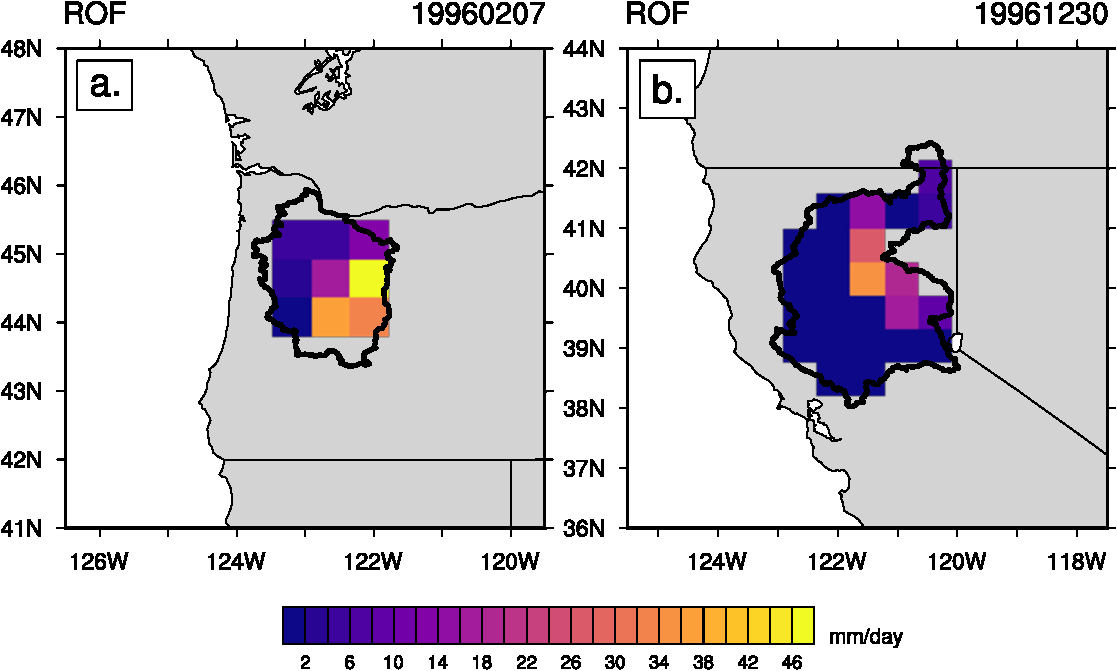
\includegraphics[width=0.7\textwidth]{figs/cropped/other_basins_ROF.pdf}
\caption{Basin shapefile domains for (a.) the Willamette River Basin (WRB) and (b.) the Sacramento River Basin (SacRB). Contoured is the surface runoff field from JRA on (a.) February 7th, 1996, and (b.) December 30th, 1996.}
\label{fig:otherbasins}
\end{figure}

To probe these events, we first acquire shapefiles defining both the WRB and SacRB, shown in Fig. \ref{fig:otherbasins}.
Like with the SRB analysis, all four datasets are masked using these basins.
Daily, basin-averaged mean timeseries are constructed with the 95\% percentiles of ROF and dSWE being computed from these distributions to use as thresholds $t_{\textrm{ROF}}$ and $t_{\textrm{dSWE}}$.
We then seek RoS events by looking for periods of concurrent PRECIP, ROF, and dSWE that all exceed relevant thresholds.

Fig. \ref{fig:ros-wrb} shows the WY96 results over the WRB. The February flood event is clearly evident in the streamflow shading along the top of the panels on the left (black colors indicating 99.9\% streamflow).
Three of the four products indicate a RoS event immediately preceding this streamflow maximum.
All products indicate spikes in PRECIP and ROF over the basin, although E3SM produces less precipitation than the other three, likely owing to its coarser resolution.
JRA has the largest and most rapid snowmelt, with both NLDAS and E3SM also showing reductions in SWE during the event.
L15 shows a small rapid increase, then a decrease in SWE during the event.
This offset is strong enough that the RoS algorithm is not triggered ($t_{\textrm{dSWE}}$ is not satisfied).
While a more detailed evaluation of the meteorology as represented by the data products is beyond the scope of this study, it is possible that some of the mechanisms discussed in Section 3.4 are also relevant in this basin.
The bubble plots on the right side of Fig. \ref{fig:ros-wrb} show a wide diversity as in Fig. 6, although the relative differences are somewhat dissimilar, implying different processes are at play, particularly for the ROF.
As before, L15 has a narrower range of dSWE over the basin (i.e., spread on the horizontal axis) but does contain large values of both precipitation (vertical axis) and runoff (marker size).
The dSWE variability for both E3SM and JRA is larger but the products generally have lower ROF and PRECIP, respectively, than both L15 and NLDAS.

\begin{figure}[H]
\centering
\begin{tabular}{@{}m{0.45\textwidth}@{\hspace{1.5em}}m{0.3\textwidth}@{}}

\begin{overpic}[width=\linewidth]{figs/cropped/L15_WillametteBasin_events.pdf}
\put (11,39.5) {\contour{white}{\large a.}}
\end{overpic}
&
\begin{overpic}[width=\linewidth]{figs/cropped/L15_WillametteBasin_scatplot.pdf}
\put (14,61.0) {\contour{white}{\large b.}}
\end{overpic}
\\
\begin{overpic}[width=\linewidth]{figs/cropped/NLDAS_WillametteBasin_events.pdf}
\put (11,39.5) {\contour{white}{\large c.}}
\end{overpic}
&
\begin{overpic}[width=\linewidth]{figs/cropped/NLDAS_WillametteBasin_scatplot.pdf}
\put (14,61.0) {\contour{white}{\large d.}}
\end{overpic}
\\
\begin{overpic}[width=\linewidth]{figs/cropped/JRA_WillametteBasin_events.pdf}
\put (11,39.5) {\contour{white}{\large e.}}
\end{overpic}
&
\begin{overpic}[width=\linewidth]{figs/cropped/JRA_WillametteBasin_scatplot.pdf}
\put (14,61.0) {\contour{white}{\large f.}}
\end{overpic}
\\
\begin{overpic}[width=\linewidth]{figs/cropped/E3SM_WillametteBasin_events.pdf}
\put (11,39.5) {\contour{white}{\large g.}}
\end{overpic}
&
\begin{overpic}[width=\linewidth]{figs/cropped/E3SM_WillametteBasin_scatplot.pdf}
\put (14,61.0) {\contour{white}{\large h.}}
\end{overpic}
\\
\end{tabular}
\caption{As in Figs. 5 (a., c., e., g.) and 6 (b., d., f., h.), except for the Willamette River Basin (WRB) during WY96. The striped gauge percentiles along the top of the left panels are derived from daily streamflow from USGS gage \#14211720 (Willamette River at Portland, Oregon).}
\label{fig:ros-wrb}
\end{figure}

Figure \ref{fig:ros-sacrb} shows the WY97 results over the SacRB.
Here, all four data products detect a RoS event in the basin in late December/early January.
The timing differs slightly between the datasets, with E3SM (L15) triggering the earliest (latest).
We speculate that this is a function of resolution, where the higher-resolution L15 contains more detailed small-scale processes (e.g., sub-basin melt at higher elevations, time for headwaters to reach the main stem).
Evaluating temporal differences at the daily scale due to model structural characteristics is an interesting target for future work.
All products capture large spikes in PRECIP and subsequent increases in ROF over the basin.
They differ more significantly in terms of dSWE, with JRA (NLDAS) producing the most (least) snowmelt over the basin.
Of note, both JRA and E3SM flag a smaller RoS event later in January while both L15 and NLDAS show increased SWE in the basin.
All products show increases in ROF, however, which coincide with a secondary maximum in the streamflow, highlighting the complexity of how surface hydrology evolves in models even if the relevant metrics (e.g., runoff) are similar.
The bubble plots on the right of Fig. \ref{fig:ros-sacrb} indicate similar behavior to Fig. \ref{fig:ros-wrb}, which is likely a function of snow processes in the SacRB being more similar to the WRB than the SRB.

\begin{figure}[H]
\centering
\begin{tabular}{@{}m{0.45\textwidth}@{\hspace{1.5em}}m{0.3\textwidth}@{}}
\begin{overpic}[width=\linewidth]{figs/cropped/L15_SacRB_USGS1802_events.pdf}
\put (11,39.5) {\contour{white}{\large a.}}
\end{overpic}
&
\begin{overpic}[width=\linewidth]{figs/cropped/L15_SacRB_USGS1802_scatplot.pdf}
\put (14,61.0) {\contour{white}{\large b.}}
\end{overpic}
\\
\begin{overpic}[width=\linewidth]{figs/cropped/NLDAS_SacRB_USGS1802_events.pdf}
\put (11,39.5) {\contour{white}{\large c.}}
\end{overpic}
&
\begin{overpic}[width=\linewidth]{figs/cropped/NLDAS_SacRB_USGS1802_scatplot.pdf}
\put (14,61.0) {\contour{white}{\large d.}}
\end{overpic}
\\
\begin{overpic}[width=\linewidth]{figs/cropped/JRA_SacRB_USGS1802_events.pdf}
\put (11,39.5) {\contour{white}{\large e.}}
\end{overpic}
&
\begin{overpic}[width=\linewidth]{figs/cropped/JRA_SacRB_USGS1802_scatplot.pdf}
\put (14,61.0) {\contour{white}{\large f.}}
\end{overpic}
\\
\begin{overpic}[width=\linewidth]{figs/cropped/E3SM_SacRB_USGS1802_events.pdf}
\put (11,39.5) {\contour{white}{\large g.}}
\end{overpic}
&
\begin{overpic}[width=\linewidth]{figs/cropped/E3SM_SacRB_USGS1802_scatplot.pdf}
\put (14,61.0) {\contour{white}{\large h.}}
\end{overpic}
\\
\end{tabular}
\caption{As in Figs. 5 (a., c., e., g.) and 6 (b., d., f., h.), except for the Sacramento River Basin (SacRB) during WY97. The striped gauge percentiles along the top of the left panels are derived from daily streamflow from USGS gage \#14211720 (Sacramento River at Verona, California).}
\label{fig:ros-sacrb}
\end{figure}

While this should only be considered a cursory investigation, it provides additional data points that the methodology can be applicable to other basins susceptible to RoS flooding.
Of note, both the WRB and SacRB contain higher and steeper orography than the SRB, implying that the algorithm can credibly detect RoS events in different basin geometries.
However, we stress a few caveats. More rigorous evaluation would be required by regional hydrologists to ensure results in other basins are hydrologically fit-for-purpose.
Further, we also acknowledge that RoS over high mountain ridges can feed into rises in streamflow in different basins (e.g., the Sierra Nevada mountains in California contribute to multiple watersheds).
Applying shapefiles containing larger hydrologic units or other spatial coverage may improve results in these regions and provide a better understanding of model variability and how land surface processes are represented in climate data.

\bibliographystyle{abbrvnat}
\bibliography{refs-ros-metrics.bib} 

\end{document}